\section{Versuch}

Der Versuchsaufbau besteht aus einer Cadmium-Lampe, die sich in einem Elektromagneten befindet.
Zur Aufnahme des Spektrums werden verschiedene optische Geräte verwendet.
Der Versuchsaufbau ist in Abbildung \ref{fig:aufbau} dargestellt.

\begin{figure}
	\centering
	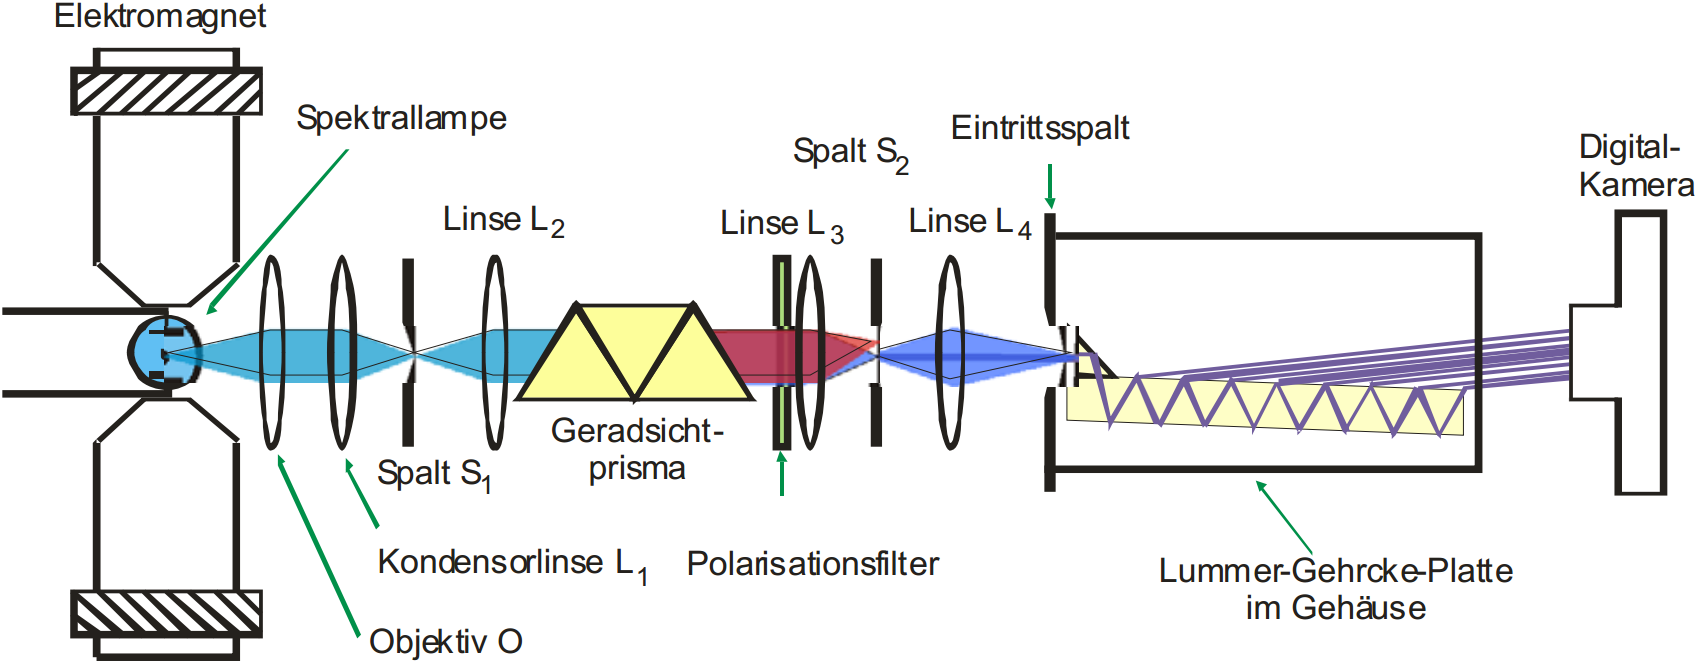
\includegraphics[width=\textwidth]{img/aufbau}
	\caption{Schematischer Versuchsaufbau \cite{v27}}
	\label{fig:aufbau}
\end{figure}

Das Licht wird zuerst durch ein Objektiv und zwei Linsen kollimiert.
Anschließend durchläuft das Licht ein Geradsichtprisma.
Das Prisma trennt die Emissionslinien der Lampe voneinander.
Die Linien werden auf eine Auswahlspalt fokussiert, den nur die gewünschte Linie passiert.

Mit einer vierten Linse wird die ausgewählte Linie auf eine Lummer-Gehrcke-Platte fokussiert.
Die Lummer-Gehcke-Platte dient dazu, Aufspaltung der Spektrallinie zu untersuchen.
Das Licht wird an der Außenwand der Platte reflektiert.
Ein Teil des Lichts verlässt dabei die Platte und interferiert.
So kann ein hohes Auflösungsvermögen erzielt werden.

Schließlich nimmt eine Digitalkamera das so erzielte Interferenzmuster auf.

Zusätzlich wird mit einer Hall-Sonde eine Messreihe für die Magnetfeldstärke in Abhängigkeit des Spulenstroms aufgenommen.
